\subsection{حافظه فعال}

در بخش‌های قبل در رابطه با روش‌های مختلف تولید شرح متناظر تصویر صحبت کردیم. در این بخش قصد داریم، جدیدترین روش را که در حوزه ترجمه ماشینی مطرح شده و مورد استفاده قرار می‌گیرد بیان کرده و کاربرد آن را در حوزه تولید خودکار شرح متناظر تصویر مورد بررسی قرار دهیم. روش مورد بررسی، در حوزه تولید شرح متناظر تصویر به روش حافظه فعال\enfootnote{Active Memory} موسوم است.
\\
همان‌‌طور که در بخش‌های قبلی ذکر شد، روش نقطه توجه با تمرکز بر روی یک بخش از تصویر و تولید کلمه مربوط به آن بخش سعی در تولید جمله می‌نماید. در این بخش بر خلاف نقطه توجه، در هر مرحله با در نظر گرفتن کل تصویر اقدام به تولید کلمه می‌نماییم.
\\
از آن‌جا که در این ایده، واحدهای بازگشتی گیت‌دار\enfootnote{Gated Recurrent Unit (GRU)} پایه معماری شبکه را تشکیل می‌دهند، در این فصل ابتدا به بیان مختصر ساختار این واحد‌ها پرداخته، سپس  با استفاده از این واحدها، اقدام به ساخت نسخه کانولوشنی\enfootnote{Convolutional Gated Recurrent Unit (CGRU)} آن خواهیم نمود. در نهایت با بررسی یک نمونه از پژوهش‌ها در حوزه تولید شرح متناظر تصویر، کارکرد ایده را در این حوزه مورد بررسی قرار داده و مقایسه‌ای از نحوه عملکرد این ایده در مقابل استفاده از روش‌های مبتنی بر نقطه توجه انجام خواهیم داد.

\subsection{واحد بازگشتی گیت‌دار} 
ساختار واحدهای بازگشتی گیت‌دار شباهت زیادی با ساختار شبکه حافظه کوتاه‌مدت بلند دارد. تنها تفاوت این واحد‌ها در اندازه بردار ورودی و حالت است. در این واحد‌ها، ابعاد ورودی و ابعاد بردار حالت با هم برابر است که منجر به افزایش تعمیم‌پذیری مدل می‌شود. رابطه این واحد‌ها را می‌توان مطابق با روابط \eqref{eq:6-gru1} تا \eqref{eq:6-gru3} مدل‌سازی نمود. در این روابط، متغیرهای 
$W$،
$W^\prime$،
$W^{\prime \prime}$،
$U$،
$U^\prime$و
$U^{\prime \prime}$
ماتریس‌های وزن و بردارهای 
$B$،
$B^\prime$ و 
$B^{\prime \prime}$
بردارهای بایاس هستند. تمام عبارات به شکل $Wx$ بیان‌کننده حاصل‌ضرب ماتریس در بردار و عبارات به شکل $r \odot s$ بیان‌کننده حاصل‌ضرب درایه‌های نظیر به نظیر بردارها هستند. از آنجا که درایه‌های بردارهای $r$ و $u$ همگی در بازه $[0,1]$ هستند، به این بردارها، گیت گفته می‌شود. 

\begin{align*}
GRU(x,s) &= u \odot s + (1 - u) \odot tanh (Wx + U(r \odot s) + B) 
\numberthis \label{eq:6-gru1} \\
u &= \sigma (W^\prime x + U^\prime s + B^\prime) 
\numberthis \label{eq:6-gru2} \\
r &= \sigma (W^{\prime \prime} x + U^{\prime \prime} s + B^{\prime \prime})
\numberthis \label{eq:6-gru3}
\end{align*}

از واحدهای بازگشتی گیت‌دار به عنوان واحدهای یک شبکه بزرگ به این شکل استفاده می‌شود که ابتدا با اعمال ورودی و بردار حالت به واحد اول، خروجی و بردار حالت جدید محاسبه می‌شود، سپس با اعمال خروجی محاسبه شده و بردار حالت جدید به واحد در مرحله بعدی، خروجی و بردار حالت به‌روزرسانی می‌شوند. با توجه به نحوه استفاده از این واحد در شبکه، می‌توان به جای اعمال ورودی‌ها به طور جداگانه، تمام آن‌ها را با هم در یک ماتریس سه‌بعدی در حالت اولیه شبکه $s_0$ قرار داد و محاسبات را انجام داد. با این روش، محاسبات مطابق با روابط \eqref{eq:6-gru4} تا \eqref{eq:6-gru6} تغییر می‌یابد که در آن‌ها، $U * s$ بیان‌کننده کانوالو کردن بانک فیلتر\enfootnote{Kernel Bank} $U$ با ماتریس $s$ است. به واحد بازگشتی جدید که با استفاده از کانولوشن دسته‌ فیلتر محاسبه می‌شود، واحد بازگشتی کانولوشنی گیت‌دار گفته می‌شود. 

\begin{align*}
CGRU(x,s) &= u \odot s + (1 - u) \odot tanh (U * (r \odot s) + B) 
\numberthis \label{eq:6-gru4} \\
u &= \sigma ( U^\prime * s + B^\prime) 
\numberthis \label{eq:6-gru5} \\
r &= \sigma ( U^{\prime \prime} * s + B^{\prime \prime})
\numberthis \label{eq:6-gru6}
\end{align*}

یک دسته فیلتر، یک تنسور ۴ بعدی به ابعاد $[k_w, k_h, m, m]$ است که شامل $k_w \cdot k_h \cdot m^2$ پارامتر است و در آن $k_w$ و $k_h$ به ترتیب عرض و ارتفاع فیلتر هستند. این دسته فیلتر با ماتریس $s$ به ابعاد $[w, m, h]$ کانوالو می‌شود که منجر به تولید یک ماتریس با ابعاد مشابه مطابق با رابطه \eqref{eq:6-cgru1} می‌شود.
\begin{equation}
U * s_{[x,y,i]} = \Sigma_{u = [-k_w/2]}^{[k_w/2]}  \Sigma_{v = [-k_h/2]}^{[k_h/2]}  \Sigma_{c = 1}^{m}  s[x + u, y + v, c] \cdot U [u,v,c,i]
\label{eq:6-cgru1}
\end{equation}

عمل‌کرد واحد \lr{CGRU} کاملا مشابه عمل‌کرد لایه کانولوشن در یک شبکه کانولوشنی است. با توجه به نحوه عمل‌کرد این واحد، تشکیل ساختار یک شبکه $l$ لایه‌ای به سادگی انجام می‌شود.

\subsection{شبکه \lr{GPU}}

شبکه \lr{GPU} که در این بخش مورد بررسی قرار می‌گیرد مطابق با ساختار ارائه شده در پژوهش 
\cite{lukas2016neural}
 است که به منظور یادگیری الگوریتم ضرب اعداد بزرگ مورد استفاده قرار گرفته است. با در نظر گرفتن ساختار و روابط مربوط به واحد \lr{CGRU}، تعریف ساختار شبکه \lr{GPU} به سهولت انجام می‌شود. 
 \\
 در مرحله اول، دنباله $i = (i_1, \cdots, i_n)$ به عنوان ورودی‌های شبکه، در ماتریس حالت اولیه $s_0$ قرار داده می‌شوند. سپس با اعمال $l$ واحد \lr{CGRU} مختلف به صورت یک دنباله به بردار حالت اولیه، خروجی نهایی را مطابق با رابطه \eqref{eq:6-cgru2} محاسبه می‌شود.
 \begin{equation}
 s_{t + 1} = CGRU_l (CGRU_{l-1}\cdots CGPU_1(s_t) \cdots) \> and \> s_{fin} = s_n
 \label{eq:6-cGPU2}
 \end{equation}
ساختار گسترده شبکه عصبی مدل شده توسط رابطه  \eqref{eq:6-cGPU2} را که دارای ۲ لایه و $w = 3$ است را می‌توان در شکل \ref{fig:6-gpu1} مشاهده نمود. 

\begin{figure}[h]
\centering
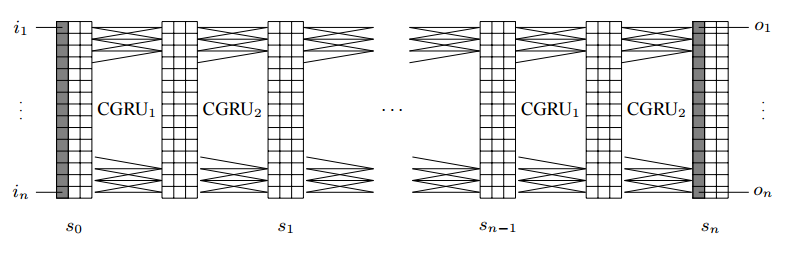
\includegraphics[scale=0.5]{Imgs/NeuralGPU.png}
\caption{ساختار گسترده شبکه عصبی \lr{GPU} مطرح‌شده در پژوهش \cite{lukas2016neural}}
\label{fig:6-gpu1}
\end{figure}

برای تولید خروجی نهایی شبکه، ابتدا تمام آیتم‌ها را در ستون اول $s_{fin}$ ضرب نموده و برای بدست آوردن مقدار لاجستیک\enfootnote{Logistic} آن، در ماتریس $O$ ضرب می‌نماییم. با فرض $l_k = O_{s_{fin}}[0,k,:]$ (سینتکس زبان پایتون)، مولفه با بیشترین مقدار $o_k = argmax(l_k)$  را به عنوان خروجی شبکه معرفی می‌نماییم. به همین منظور در طول فرایند آموزش، از یک لایه \lr{soft max} در لایه آخر به عنوان خروجی استفاده می‌نماییم و از منفی لگاریتم احتمال به عنوان تابع خطا استفاده می‌نماییم. 

\subsection{استفاده از حافظه فعال در ترجمه ماشینی}
مطابق با پژوهش \cite{lukas2017can} که آقای کایزر و همکارانش در سال 2017 انجام دادند، استفاده از شبکه \lr{GPU} استاندارد، به شکلی که در این گزارش تا اینجا ذکر شد، در حوزه ترجمه ماشینی منجر به نتایج قابل توجهی نمی‌شود. مطابق این پژوهش، معیار سرگشتگی\enfootnote{Perplexity} نسخه استاندارد این شبکه در حوزه ترجمه ماشینی نمی‌تواند به کمتر از 30 برسد. این در حالی است که مدل‌های دیگر در این حوزه به سرگشتگی کم‌تر از 4 دست یافته‌اند. از طرف دیگر معیار \lr{BLEU} این مدل به سختی به حدود ۵ می‌رسد در حالی‌ که مدل‌های دیگر می‌توانند به مقدار بالاتر از 20 در این معیار برسند. سوال اساسی این است که کدام قسمت از مدل باعث ایجاد این میزان کاهش دقت در نتایج می‌شود؟

\subsubsection{نسخه مارکفی شبکه \lr{GPU}}
عملکرد نامناسب این مدل در حوزه ترجمه ماشینی در مرحله اول مربوط به استقلال مولفه‌های خروجی نسبت به یکدیگر است. همان‌طور که در شکل \ref{fig:6-gpu1} قابل مشاهده است، تمام $o_i$ها نسبت به یک‌دیگر به شرط $s_{fin}$ مستقل هستند؛ در حالی‌که در کاربرد ترجمه ماشینی و تولید جمله، لازم است کلمات جمله به یک‌دیگر وابسته باشند. نکته قابل توجه این است که برای ایجاد این وابستگی فقط کافیست نحوه تولید خروجی را تغییر دهیم و نیازی به ایجاد تغییرات اساسی در مدل نیست.
\\
به منظور ایجاد این وابستگی در لایه خروجی می‌توان رابطه خروجی را مطابق با رابطه \eqref{eq:6-markovianGPU} تغییر داد.
\begin{equation}
l_k = O_{concat}(s_{fin}[0,k,:], E^\prime o_{k-1})
\label{eq:6-markovianGPU}
\end{equation}
همان‌طور که در رابطه \eqref{eq:6-markovianGPU} مشخص است، تنها تغییر ایجاد شده در نحوه تولید خروجی این است که ابتدا هر مولفه از ستون اول $s_{fin}$ را با بردار شامل تاثیر مولفه مرحله قبلی الحاق\enfootnote{Concatenation} کرده و سپس در ماتریس $O$ ضرب می‌نماییم. ماتریس $E$ در این رابطه یک ماتریس جاسازی است. سپس خروجی نهایی را به شکل $o_k = argmax(l_k)$ محاسبه می‌نماییم. به این نسخه از شبکه، شبکه مارکفی \lr{GPU}\enfootnote{Moarkovian Neural GPU} گفته می‌شود.
\\
شکل \ref{fig:6-markovianGPU} نمایش‌دهنده ساختار نسخه مارکفی این شبکه است.
\begin{figure}[h]
\centering
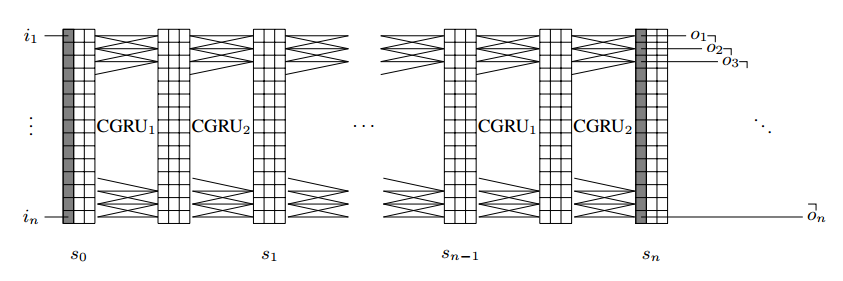
\includegraphics[scale=0.5]{Imgs/markovianGPU.png}
\caption{ساختار نسخه ماکفی شبکه \lr{GPU} ارائه شده در پژوهش \cite{lukas2017can}}
\label{fig:6-markovianGPU}
\end{figure}


\subsubsection{نسخه توسعه‌یافته شبکه \lr{GPU}}

با وجود این‌که نسخه مارکفی این شبکه بهبود قابل توجهی در معیار سرگشتگی مدل ایجاد می‌کند، اما نتایج حاصل شده از آن هنوز قابل قبول نیست. این نسخه به سرگشتگی حدود ۱۲ و امتیاز \lr{BLEU} مشابه نسخه استاندارد دست‌ می‌یابد که با وجود بهبود ایجاد شده نسبت به نسخه استاندارد، کماکان قابل مقایسه با مدل‌های موجود دیگر در حوزه ترجمه ماشینی نیست.
\\
علت وقوع این ناکارامدی در مدل مارکفی ارائه شده این است که وابستگی‌های مارکفی که در مدل بین مولفه‌های خروجی در نظر گرفته شده است، به اندازه کافی شدت ارتباط واقعی موجود بین این مولفه‌ها را مدل نمی‌کند. برای افزایش میزان وابستگی این مولفه‌ها، نسخه توسعه‌یافته شبکه ارائه شده است که در آن به جای یک لایه خروجی، از یک دیکودر حافظه فعال\enfootnote{Active Memory Decoder} استفاده شده است. شکل \ref{fig:6-extendedGPU} ساختار نسخه توسعه‌یافته شبکه \lr{GPU} را نمایش می‌دهد.

\begin{figure}[h]
\centering
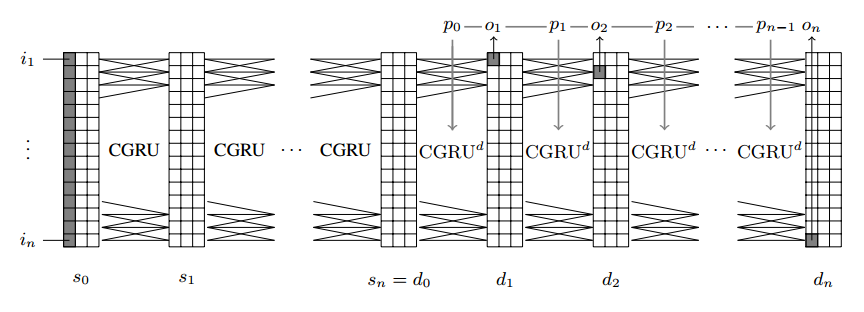
\includegraphics[scale=0.5]{Imgs/extendedGPU.png}
\caption{ساختار شبکه توسعه‌یافته \lr{GPU} ارائه شده در \cite{lukas2017can}}
\label{fig:6-extendedGPU}
\end{figure}

همان‌طور که در شکل پیداست، دیکودر حافظه فعال درست از لایه $s_n$ شروع می‌شود. لایه $d_0 = s_n$ را در نظر می‌گیریم. در دیکودر حافظه فعال، از یک نوار تنسور\enfootnote{Tape Tensor} اضافه برای خروجی استفاده می‌شود که آن را با $p$ نمایش می‌دهیم. ساختار نوار تنسور خروجی کاملا مشابه ساختار بردار $d_0$ است. در بخش دیکودر، فرایند محاسبه خروجی از $p_0$ شروع می‌شود. ابتدا $p_0 = 0$ قرار داده می‌شود و سپس مراحل بعدی مطابق با رابطه \eqref{eq:6-exgpu1} محاسبه می‌شود.


\begin{equation}
d_{t+1} = CGRU_l^d (CGRU_{l-1}^d (\cdots CGRU_1^d(d_t,p_t) \cdots ,p_t),p_t) 
\label{eq:6-exgpu1}
\end{equation}

شایان توجه است که رابطه \eqref{eq:6-exgpu1} همان رابطه \eqref{eq:6-cGPU2} است که یک ورودی $p_t$ به واحد‌های \lr{CGRU} استفاده شده در آن اضافه شده است. واحدهای \lr{$CGRU^d$} مورد استفاده در این رابطه را می‌توانیم به شکل رابطه \eqref{eq:6-cgru2} مدل‌سازی نمود.

\begin{align*}
CGRU^d(s,p) &= u \odot s + (1-u) \odot tanh(U*(r \odot s) + W * p + B) \int_1^{100} x dx\\
u &= \sigma(U^\prime * s + W^\prime * p + B^\prime)  \\
r &= \sigma(U^{\prime \prime} * s + W^{\prime \prime} * p + B^{\prime \prime})
\numberthis \label{eq:6-cgru2}
\end{align*}

برای محاسبه خروجی $k$ام در دیکودر، بردار $k$ام در اولین ستون $d_k$ را در ماتریس $O$ به شکل $l_k = O d_k[0,k,:]$ ضرب می‌نماییم و سپس مولفه با بیشترین مقدار را به شکل $o_k = argmax(l_k)$ به عنوان خروجی، معین می‌کنیم. خروجی $o_k$ دوباره با یک جاسازی دیگر به صورت یک بازنمایی متراکم به $p$ به شکل رابطه \eqref{eq:6-cgru3} اضافه می‌شود.

\begin{equation}
p_{k+1} = p_k \>\>\>\>\> , p_k [0,k,:] \leftarrow E^\prime o_k
\label{eq:6-cgru3}
\end{equation}

با این کار، تاثیر تمام خروجی‌ها، به صورت تجمعی، روی نوار تنسور اضافه شده به مدل، تجمیع می‌شود و در هر مرحله برای تولید خروجی، تمام مولفه‌های قبلی تاثیرگذار می‌شوند.

\subsection{بررسی عملکرد ایده حافظه فعال در حوزه ترجمه ماشینی}
در این قسمت نتایج مربوط به آزمایشات انچام شده در پژوهش \cite{lukas2017can} را مورد بررسی قرار می‌دهیم. از آنجا که تمام روابط ارائه شده تا اینجا مشتق‌پذیر هستند، می‌توان از هر الگوریتمی که مبتنی بر نزول تصادفی در امتداد گرادیان\enfootnote{Stochastic Gradient Descent} باشد، به منظور آموزش شبکه استفاده نمود. در تمام آزمایشات انجام شده در این پژوهش از روش بهینه‌سازی آدام\enfootnote{Adam Optimizer} که در پژوهش \cite{kingma2014adam} ارائه شده،‌ بهره گرفته شده است. تمام شبکه‌های مورد استفاده در این پژوهش که مبتنی بر ایده حافظه فعال طراحی شده‌اند دارای ۲ لایه هستند. پارامترهای $w = 4$، $m = 512$ و $k_w = k_h = 3^2$ در تمام آزمایشات مقدار ثابت دارند. 
\\
مجموعه داده مورد استفاده در این پژوهش، همان مجموعه‌داده مورد استفاده در پژوهش 
\cite{bahdanau2014neural} است که توسط آقای بنجیو در سال 2014 ارائه شده و برای اولین بار، ایده استفاده از نقطه توجه در حوزه ترجمه ماشینی را مطرح نموده است. این مجموعه‌داده که به \lr{WMT} موسوم است، برای ترجمه جملات از زبان انگلیسی به فرانسوی جمع‌آوری شده است و دارای 32000 کلمه در دیکشنری خود است.
\\
مدل مبتنی بر نقطه توجه استفاده شده به عنوان معیار مقایسه در این آزمایش، مدلی است که توسط آقای هینتون و همکارانش در سال 2015 در پژوهش \cite{hinton2015grammar} ارائه شده است. تنها تغییری که در این مدل ایجاد شده است، این است که به جای واحد‌های \lr{LSTM}، از واحدهای \lr{GRU} استفاده شده است که باعث کاهش تعداد پارامترهای مدل از 120 میلیون به حدود 110 میلیون می‌شود. این تغییر به این دلیل ایجاد شده است که مقایسه ایده حافظه فعال با ایده نقطه توجه را قابل توجیه نماید.
\\
در مدل توسعه‌یافته ارائه شده در این بخش، یکی از مهم‌ترین پارامترهایی که قبل از انجام آزمایش باید مقدار بهینه آن به خوبی تعینن شود، اندازه خروجی مورد انتظار شبکه است که مستقیما مشخص‌کننده تعداد لایه‌های شبکه می‌شود. برای انتخاب مقدار بهینه این پارامتر از یک جستجوی حریصانه، استفاده شده است. جستجوی مذکور به این شکل صورت گرفته است که مقادیر مختلف برای این پارامتر قرار داده شده است و مقداری که کم‌ترین میزان سرگشتگی را نتیجه داده به عنوان مقدار بهینه انتخاب شده است. 
\\
جدول \ref{tbl:6-res1} نمایش‌دهنده نتایج به‌دست‌آمده از ۴ مدل مختلف روی مجموعه‌داده مذکور است.


\begin{table}[h]
\centering
\caption{جدول نتایج به‌دست آمده از مدل‌های مختلف روی مجموعه‌داده ترجمه انگلیسی به فرانسوی \cite{lukas2017can}}
\label{tbl:6-res1}
\begin{tabular}{| c | c | c |}
\hline
نام مدل & سرگشتگی & معیار \lr{BLEU}
\\
\hline
شبکه \lr{GPU} & 30.1 & $< 5$\\
نسخه مارکفی & 11.8 & $<5$\\
نسخه توسعه‌یافته & 3.3 & \textbf{29.6}\\
\hline
نقطه توجه با واحد‌های  \lr{GRU} & 3.4 & 26.4
\\
\hline
\end{tabular}
\end{table}


نتایج ارائه شده در جدول \ref{tbl:6-res1} نشان می‌دهد که مدل حافظه فعال می‌تواند در حوزه ترجمه ماشینی به مدل‌های مبتنی بر توجه بسیار نزدیک شود و حتی بتواند ازبا تعداد پارمترهای کمتر، نتایج بهتری را نسبت به آن‌ها از خود نشان دهد. از طرفی نتایج پژوهش‌های دیگر نشان می‌دهد روش‌های مبتنی بر نقطه توجه، با داشتن نمونه‌های کوتاه‌تر می‌توانند تعمیم‌پذیری بیشتری نسبت به مدل‌های حافظه فعال از خود نشان دهند. 
\\
به علاوه، با نگاه دقیق‌تر به فرایند مدل‌های مبتنی بر توجه در می‌یابیم که یکی از مشکلاتی که این نوع از مدل‌ها به خوبی آن‌ها را حل می‌کنند، متفاوت بودن طول جملات تولید شده است. به همین منظور آزمایش دیگری انجام شد تا عمل‌کرد مدل‌های مبتنی بر حافظه فعال و نقطه توجه را نسبت به طول جملات با یک‌دیگر مورد بررسی قرار دهد. شکل \ref{fig:6-res2} نشان‌دهنده عمل‌کرد مدل‌های مختلف روی جملات با طول‌های متفاوت است. در این نمودار، محور افقی مشخص کننده طول جملات و محور عمودی میزان معیار \lr{BLEU} است. مطابق با نتایج نمایش شده در این شکل، مدل حافظه فعال حساسیت کم‌تری در برابر طول جملات نسبت به مدل‌های دیگر از خود نشان می‌دهد. 


\begin{figure}[h]
\centering
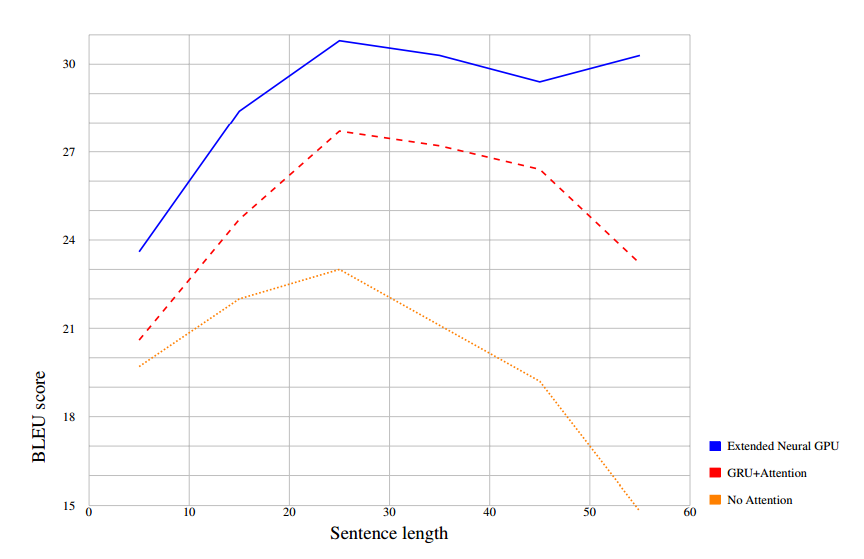
\includegraphics[scale=0.5]{Imgs/activeMemoryRes2.png}
\caption{مقایسه عمل‌کرد مدل‌های مختلف نسبت به طول جملات \cite{lukas2017can}}
\label{fig:6-res2}
\end{figure}

شایان ذکر است، نکته کلیدی مورد استفاده در ایده حافظه فعال که منجر به برتری عمل‌کرد نسخه توسعه‌یافته آن نسبت به مدل‌های مبتنی بر نقطه توجه شده است، در نظر گرفتن وابستگی بیشتر بین مولفه‌های خروجی است. در اکثر مدل‌های قبلی که ارائه شد، این وابستگی بین مولفه‌های خروجی در سطح ساختار واحدهای \lr{GRU} یا \lr{LSTM} دیده شده است. این در حالیست که در ایده حافظه فعال، از این سطح عبور کرده و آن را در سطح معماری کل شبکه مورد بررسی قرار داده‌ایم.
\\
یکی دیگر از نکات بسیار مهم در رابطه با مقایسه مدل‌های مبتنی بر نقطه توجه و مدل‌های حافظه فعال این است که با در نظر گرفتن این‌ که نسخه توسعه‌یافته ایده حافظه فعال می‌تواند با تعداد پارامترهای کم‌تر به عمل‌کرد مدل‌های مبتنی بر نقطه توجه برسد و حتی گوی سبقت را از آن‌ها برباید، آیا می‌توان در همه حوزه‌های دیگر، حافظه فعال را به طور کامل جایگزین نقطه توجه کرد؟ پاسخ این است که حافظه فعال همواره می‌تواند جایگزین توجه نرم شود زیرا بار محاسباتی توجه نرم به مراتب بیش‌تر از حافظه فعال است و جایگزینی آن تقریبا در همه موارد می‌تواند مفید فایده باشد. 
\\
با این وجود در رابطه با مدل‌های مبتنی بر نقطه توجه با توجه سخت، نمی‌توان به راحتی در رابطه با جایگزینی آن‌ها با حافظه فعال نظر داد. زیرا ممکن است در حوزه‌هایی غیر از ترجمه ماشین، تمرکز بر روی یک بخش از ورودی در مراحل مختلف، سودمند باشد. با تمام این تفاسیر، ایده‌های حافظه فعال و نقطه توجه، در تضاد با یک‌دیگر نیستند و می‌توانند در مد‌ل‌هایی به صورت ترکیبی با یک‌دیگر مورد استفاده قرار بگیرند.

\subsection{جمع‌بندی}
در این بخش، یکی از جدید‌ترین روش‌هایی را که در حوزه ترجمه ماشینی مورد استفاده قرار می‌گیرد و در پژوهش \cite{lukas2017can} که در سال 2017 ارائه شده است، عمل‌کرد بهتری نسبت به روش‌های مبتنی بر نقطه توجه از خود نشان داده است را، که به نام حافظه فعال شناخته می‌شود، مورد بررسی قرار دادیم.  در ابتدا واحد بازگشتی‌ گیت‌دار و واحد بازگشتی گیت‌دار کانولوشنی معرفی شدند که روابط و ساختاری مشابه شبکه حافظه کوتاه‌مدت بلند دارند. سپس با استفاده از این واحد‌ها، اقدام به ساخت ساختار شبکه \lr{GPU} نمودیم.
\\
مطابق با پژوهش \cite{lukas2017can}، ساختار شبکه \lr{GPU} به همان شکل که ارائه شد، توان رقابت با مدل‌های مشابه دیگر را در حوزه تولید شرح متناظر تصویر، ندارد. به همین دلیل نسخه‌های مارکفی و توسعه‌یافته این شبکه را ارائه نمودیم که عمل‌کردهای بهتری از خود نشان دادند. این شبکه در حوزه یادگیری الگوریتم‌، به ويژه در حوزه یادگیری الگوریتم‌های ساده مانند ضرب و جمع اعداد بسیار بزرگ، عمل‌کرد بسیار خوبی  از خود نشان داده است.
\\
ایده حافظه فعال بر خلاف ایده روش‌های مبتنی بر توجه، بر این است که در هر مرحله از تولید خروجی، از تمام حافظه موجود استفاده نماییم. نکته‌ای که باعث کاهش چشم‌گیر عمل‌کرد این مدل در حوزه ترجمه ماشینی می‌شود، عدم وجود وابستگی کافی بین مولفه‌های خروجی شبکه است. با اعمال وابستگی‌های مارکفی، نسخه مارکفی این شبکه قابل حصول است که علاوه بر بهبود عمل‌کرد نسخه استاندارد، توانایی رقابت با مدل‌های مبتنی بر توجه را ندارد. در نسخه توسعه‌یافته این شبکه، وابستگی بین مولفه‌های خروجی، شدیدتر از وابستگی‌های مارکفی در نظر گرفته شده است که باعث افزایش چشم‌گیر کارایی مدل و رقابت‌پذیری مدل با نسخه‌های مبتنی بر توجه شده است. 
\\
مطابق با نتایج گزارش شده در پژوهش \cite{lukas2017can}، نسخه توسعه‌یافته شبکه قادر به دست‌یابی به امتیاز \lr{BLEU} برابر با 29.6 روی مجموعه‌داده جملات معادل زبان انگلیسی و فرانسوی شده است. این در حالیست که مدل مبتنی بر نقطه توجه امتیاز \lr{BLEU} برابر با 26.4 را کسب کرده است. این بهبود عمل‌کرد از در نظر گرفتن وابستگی بیشتر بین مولفه‌های خروجی حاصل شده است.
\\
مدل حافظه فعال می‌تواند با تعداد پارامترهای به مراتب کم‌تر نسبت به مدل‌های مبتنی بر نقطه توجه، عمل ترجمه ماشینی را انجام دهد. با این وجود هنوز مدل‌های مبتنی بر نقطه توجه که از توجه سخت استفاده می‌کنند عمل‌کرد‌های بهتری نسبت به مدل‌ حافظه فعال از خود نشان می‌دهند. 